% Intended LaTeX compiler: pdflatex
\documentclass[11pt]{article}
\usepackage[utf8]{inputenc}
\usepackage[T1]{fontenc}
\usepackage{graphicx}
\usepackage{grffile}
\usepackage{longtable}
\usepackage{wrapfig}
\usepackage{rotating}
\usepackage[normalem]{ulem}
\usepackage{amsmath}
\usepackage{textcomp}
\usepackage{amssymb}
\usepackage{capt-of}
\usepackage{hyperref}
\usepackage{minted}
\author{Sandy Urazayev\thanks{ctu@ku.edu}}
\date{}
\title{Selected Final Projects\\\medskip
\large Embedded Systems}
\hypersetup{
 pdfauthor={Sandy Urazayev},
 pdftitle={Selected Final Projects},
 pdfkeywords={},
 pdfsubject={},
 pdfcreator={Emacs 28.0.50 (Org mode 9.3)}, 
 pdflang={English}}
\begin{document}

\maketitle
\tableofcontents


\section{Web Server Car by Embedheads}
\label{sec:org5a6634c}
\textbf{Sandy Urazayev} and \textbf{KayLee Mitchell}

\begin{enumerate}
\item Motivation
\label{sec:org3c18a1a}
After completing the standard milestones, Kaylee and I were out for blood. We
wished to do something fun and daring. A way to combine the past and the
future into a single project; let it breathe a little. We came to an idea of
writing our car in C/Assembly and making the controls with HTML/Python.

\item Design
\label{sec:org27cae87}
The design is incredibly simple. We utilize the basic motor control functions
written in C that we used in milestones 1-3; we add a couple more functions,
such as \texttt{reverse}, \texttt{steering}, and \texttt{angle}. And we would need a webserver that
listens to any incoming HTTP connections to send commands through the serial
to our motor controller. Finally, some simple HTML page to make the web
server endpoints call more bearable. The design schematic would look like:

\begin{verbatim}
  -------      +------------+  	 +-----------+
 (  user )-----+ HTML Page  +----+ Web Server|
  -------      +------------+  	 +-----+-----+
				       |
			   Serial ---> |
				       |
 -------      +----------------+   +---+----+
( Metal )-----+     Motor      +---+ HiFive |
 -------      |   Controller   |   +--------+
	      +----------------+
\end{verbatim}
\end{enumerate}

\section{Bluetooth-Controlled Car by Big Dogs}
\label{sec:org7905014}
\textbf{Connor Sutton} and \textbf{Aidan Schmelzle}

\begin{enumerate}
\item Motivation
\label{sec:org6cb8027}
We felt that adding a method of manually maneuvering our car would be a great
way to elevate our project, and it was something that would be a lot of fun
to play around with. For many, remote-controlled cars are a source of
childhood nostalgia, and to implement that functionality ourselves was a very
exciting idea. We also felt that we had all the means and resources necessary
to accomplish the task.

\item Design
\label{sec:orgee758d2}
At first, the implementation seemed like it would be quite trivial. In the base
project, the Raspberry PI sends information from the neural network to the
Hi-five board through the UART, and this information is interpreted to
manipulate the motors that control the car’s movement. All we had to do was
write a python file that sends information to the UART in the same way, except
that the source of this information would be inputs from the controller rather
than the output of the neural network. The most daunting task was to set up the
Bluetooth connection between the controller and the Raspberry Pi.

\item Implementation
\label{sec:org769f23a}
At first, our implementation went according to plan. We encountered some
major, unexpected hardships, however, when we were trying to use the
information received by the HiFive to actually manipulate the motors. We
could get the steering angle to change correctly, but trying to change the
speed of the car resulted in all sorts of weird, seemingly inexplicable
errors, and the more we tried to fix it, the weirder our issues became. In
trying to solve our problem, others arose, and soon even the steering stopped
working. When it was our turn to demo, we were essentially back at square one
and in trouble.

\item Results
\label{sec:org7b45eeb}
In a miraculous display of dedication and willpower, Aidan solved the
mysterious issues preventing our car from operating, and we were able to
successfully demo our project. We learned a lot about working with hardware
and bare-metal programming through this project. It also reinforced the fact
that implementation of an idea is hardly ever as simple as it sounds, but in
the end, the difficulty increases our understanding and heightens the sense
of reward and accomplishment.

\begin{center}
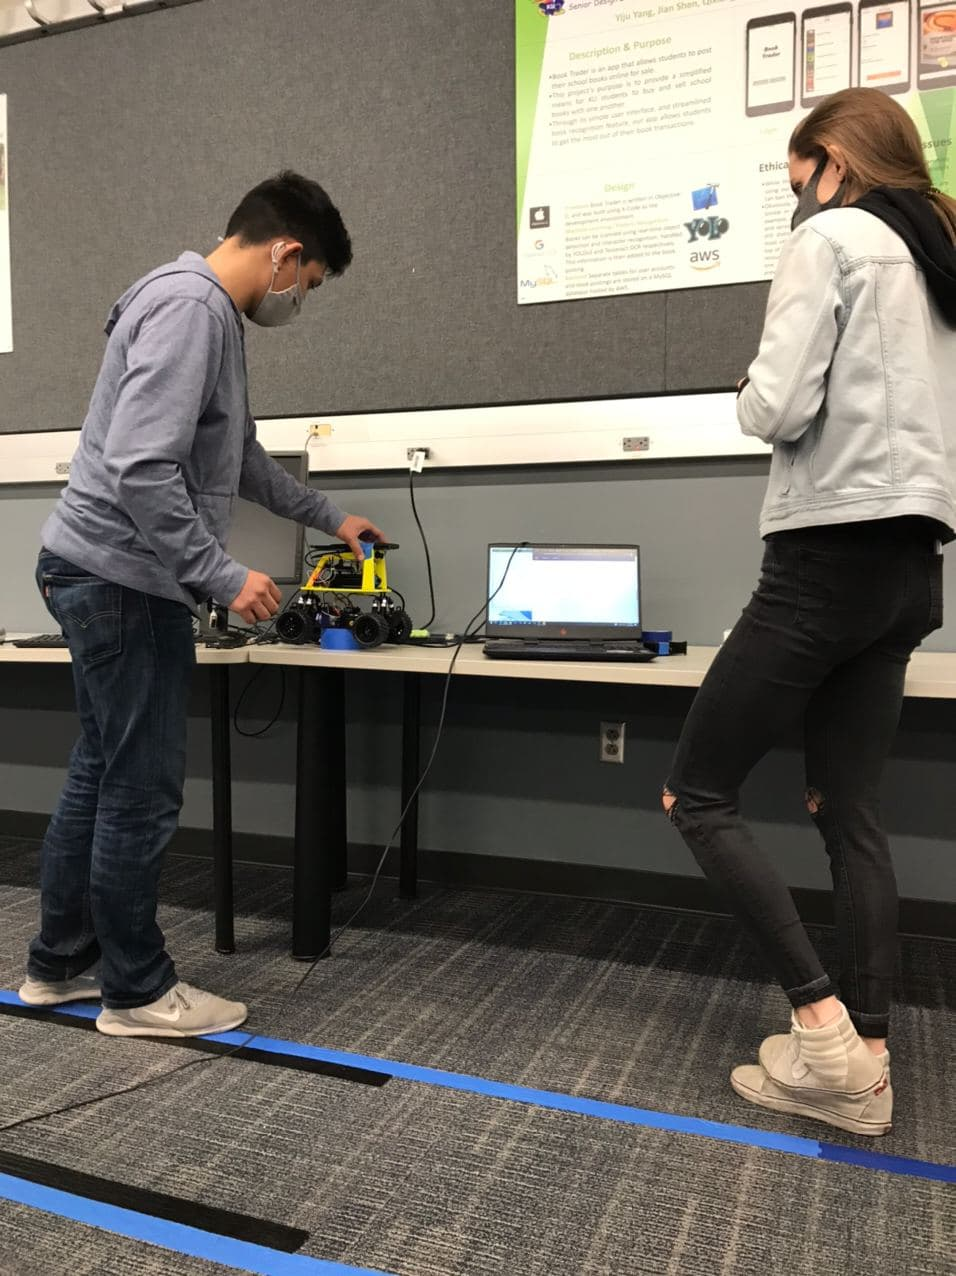
\includegraphics[width=.9\linewidth]{./bluetooth_1.jpg}
\end{center}

\begin{center}
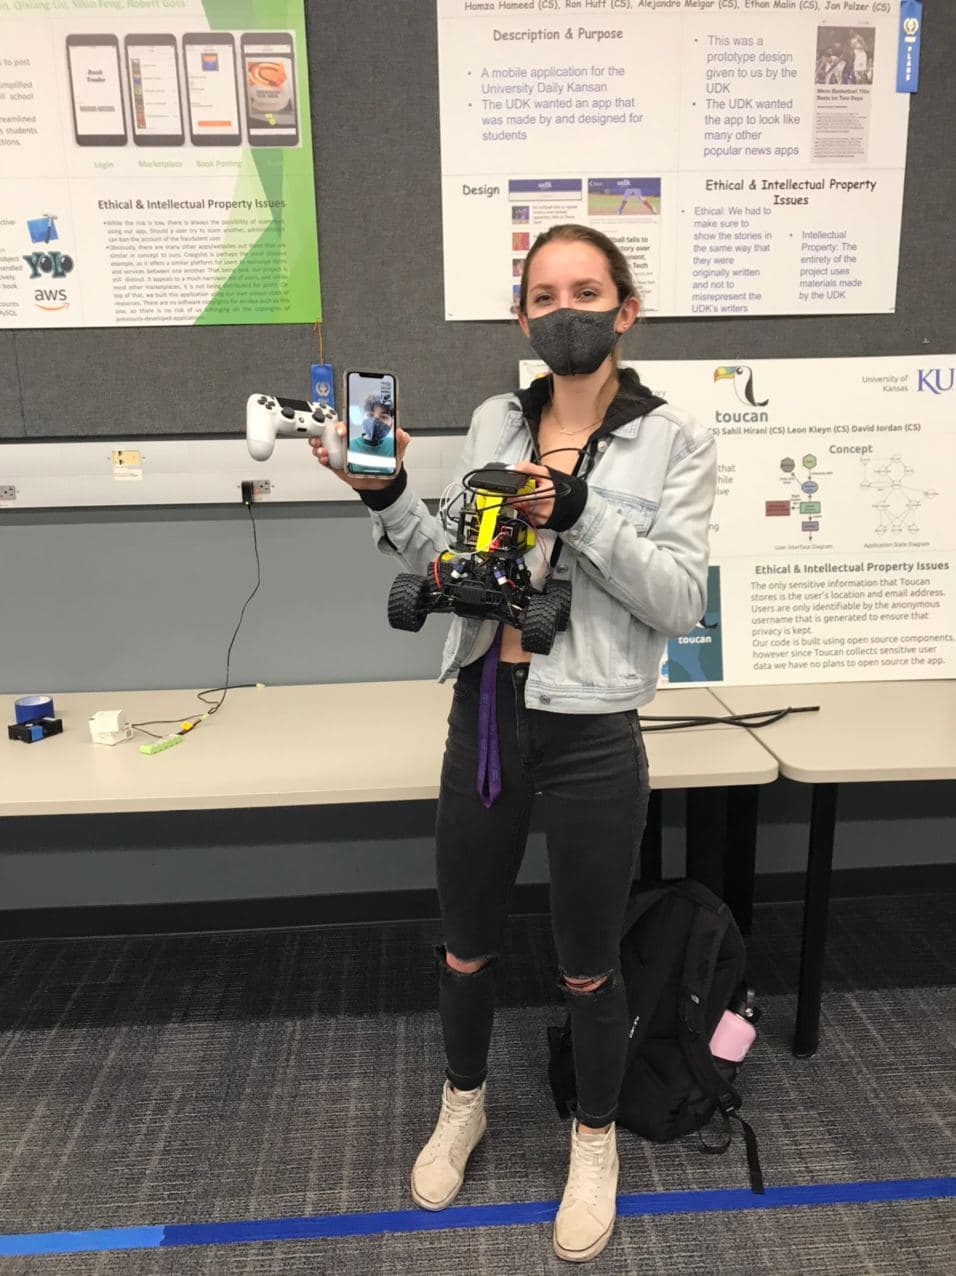
\includegraphics[width=.9\linewidth]{./bluetooth_2.jpg}
\end{center}
\end{enumerate}


\section{Reversing Anti-collision Blinker Car by Black Box}
\label{sec:org6807d00}
\textbf{Jonelle Gamble} and \textbf{Abdoul Diallo}

\begin{enumerate}
\item Motivation
\label{sec:org3f5c129}
One of the main motivations while doing this lab was to put our
knowledge of programming into practice. We learned some C programming
during lectures, that added to prior knowledge of C++, and it was a
fun project to work on. We were able to see our code’s effects not
only through monitors but making an object move/stop (the
car). Another thing is that we learned a lot while doing this project,
because we had to deal with many areas, we had not been exposed to
prior to taking this class.

\item Design
\label{sec:org546d5ac}
We initially thought, for the reverse function of the car, we only
had to set the speed to reverse to get it to work properly. For the
anti-collision, our initial thoughts were to write code similar to
lab 3 that gets information form the lidar sensor. However, instead
of changing the light on the HiFive Board, we would call the stop
car function when an object is detected 75cm away. Lastly, our
initial thoughts for blinker lights were to put together what we
learned in lab 4 and 5 where we blinked lights different colors and
used interrupts. We also knew that we would need an if statement to
check whether the steering was turning right or left (-45 to 0 or 0
to 45 degrees) and change the color of the light accordingly.

\item Implementation
\label{sec:org4d92b5e}
We changed the reverse function to match the graph that was shown
by the TAs, because the reverse option of the cars are locked when
they go forward. We implemented something called a double click to
decrease the speed of the car slowly to the reverse, then back to
neutral, before setting it slowly to the reverse speed again. The
hardship encountered while testing the reverse function is that the
cars needed to be calibrated at start. The last speed run by car
before it turns off is set as the neutral on the next start. As for
the Lidar, our initial thoughts were correct. However, we spent
some time trying to set up the UARTS on the HiFive, since one was
used by the Pi already. The pins were also inverted on the board
for the connections. Moreover, the delays in the main function made
it so the Lidar was sending information later than it should for
the car to stop at the right moment. The blinker also complained
because of delays and the position of the code for the interrupts
inside the main function mattered. We made it work by updating a
variable which handled the led index to turn on according to the
degree of the steering angle. We also had to remove and put back
the code for a version specification in the Pi, because the
Raspberry Pis have different software versions. We wanted to
implement a remote controller with Bluetooth, but we couldn’t get a
controller.

\item Results
\label{sec:orgcd361e5}
Our code worked when we showed it to TAs during lab, however, when
demoing it we had to change the code to make the camera work,
because we were given a car with a different OS version for the
Pi. We also needed to add delays in so that the TAs could calibrate
the car before it starts running. For the results of our demo,
everything worked correctly except our blinkers were not blinking
at the correct rate/frequency. We think that this project was a lot
more challenging compared to the previous labs, however, it was
very rewarding due to the knowledge we gained.

\begin{center}
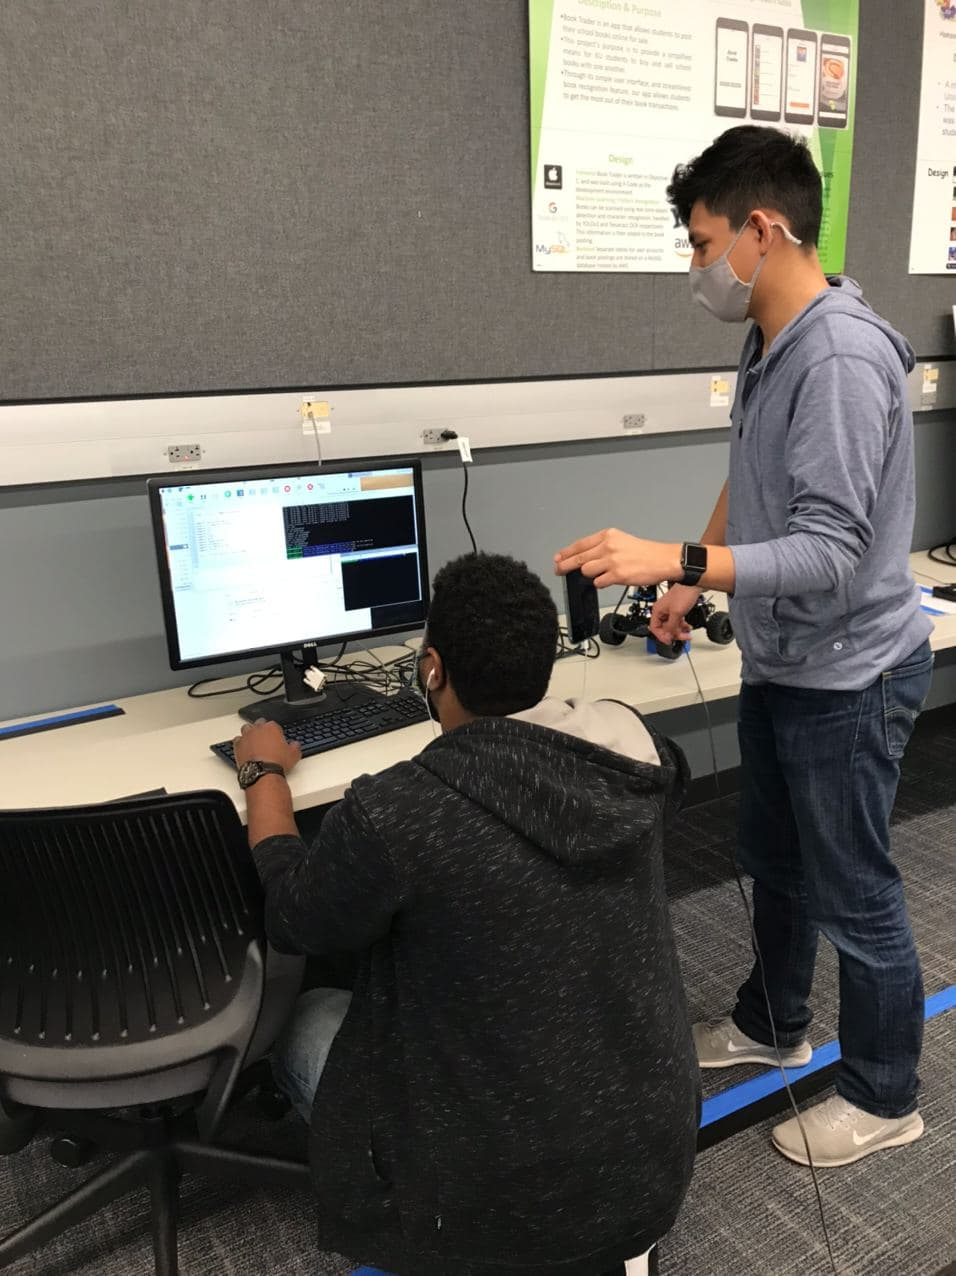
\includegraphics[width=.9\linewidth]{./anticol_1.jpg}
\end{center}

\begin{center}
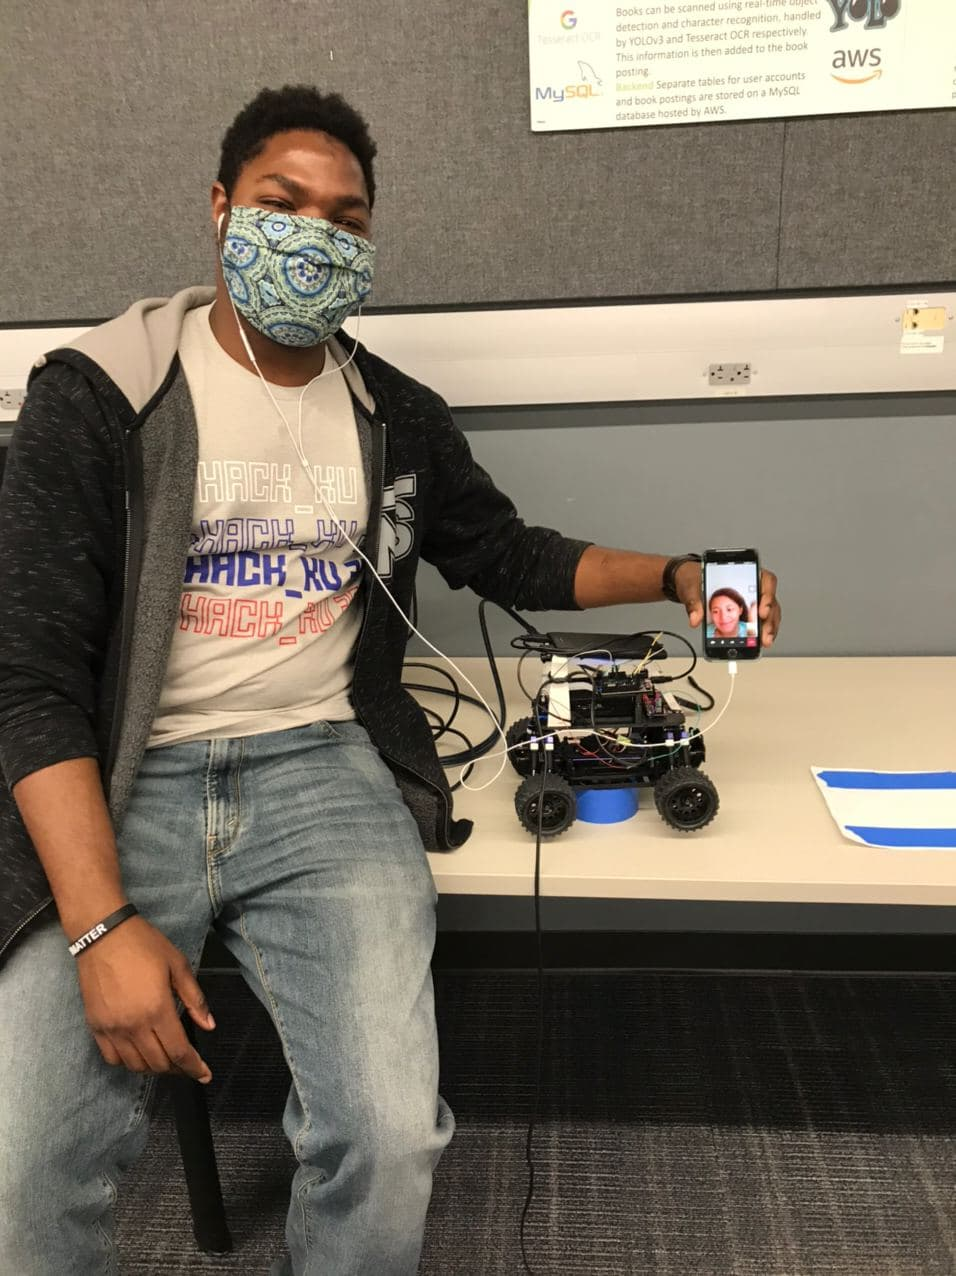
\includegraphics[width=.9\linewidth]{./anticol_2.jpg}
\end{center}
\end{enumerate}


\section{Self-Guided Car with a memory by Jeng-Atkins}
\label{sec:org8bff800}
\textbf{Joshua Jeng} and \textbf{Thomas Atkins}

\begin{enumerate}
\item Motivation
\label{sec:org2371122}
Having implemented Milestones 1-3 in a relatively streamlined fashion, we
were each looking for a challenge for Milestone 4. We each took a task and
implemented it, with Thomas taking the course mapping and Joshua trying to
implement the collision avoidance task.

\item Design
\label{sec:org231b52b}
In Lab 3, we had implemented range detection using a LIDAR sensor connected
to a Hifive board through UART 0. Thus, it seemed simple to transfer that
code over and modify it to use UART 1 and stop the motor when within range of
an obstacle. For the course mapping portion we planned on just creating a log
in memory of what was being sent to the car and then writing it to a file to
be read later.

\item Implementation
\label{sec:orgb6c0902}
For the LIDAR, initially, it seemed that the implementation process would be
as simple as copying the code from Lab 3 into the project, and modify it to
use UART 1 rather than UART 0, as was used back then. However, this ended up
proving extremely challenging. Debugging showed that the code worked when
using UART 0, hinting that the problem lay deeper than our code. From there,
switching boards, double-checking the Hifive pinouts, and so forth yielded no
insight into the ultimate cause of the issue.

The course mapping implication unutilized two different files for the mapping of
the course and the repeating the course. This was done to avoid the hassle of
having two have a command line switch and two different branches in the main
loop. In the writing we simply left the script mostly the same and only added a
few time checks and logged the info. The log file consisted of the angle that
was sent to the car and time information about when it started to go at that
angle and then when it switched to a new angle. The reading file required more
work to get up and running as it required rewriting most of the main loop to
check the values in the log file instead of inference from the camera.

\item Results
\label{sec:org0bbc52a}
The main demonstration on the track was apparently very successful. While the
actual self-driving was rather suspect, the car did attempt to make the
correct adjustments based on the camera input. Due to the aforementioned
issues with the LIDAR, the collision avoidance extra credit was never
tested. The course mapping aspect of milestone 4 was successful. We were able
to replicate the angel sent to the HiFive board during our demonstration.

\begin{center}
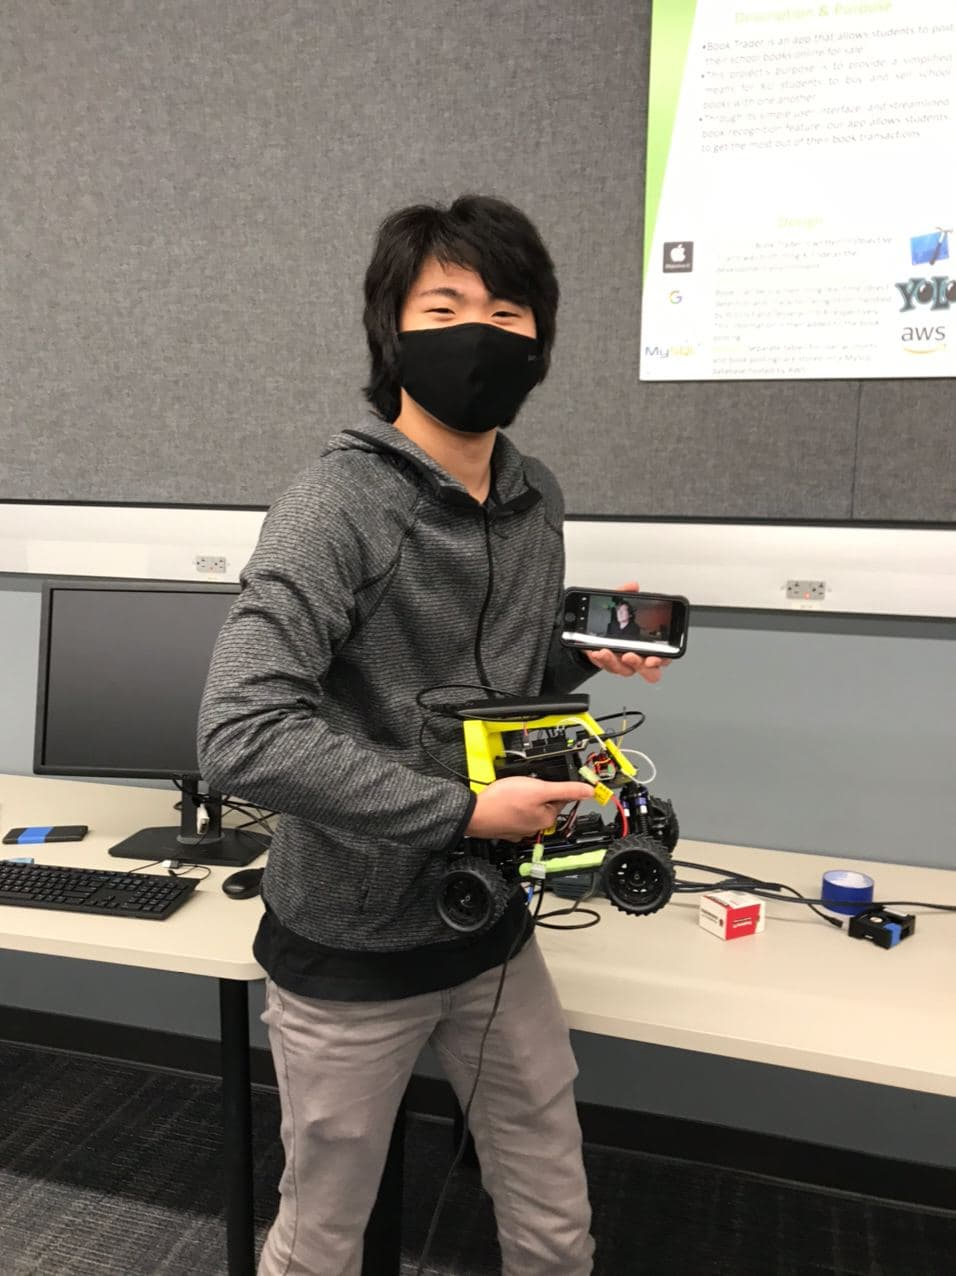
\includegraphics[width=.9\linewidth]{./jengatkins_1.jpg}
\end{center}
\end{enumerate}
\end{document}
